% !TeX root = ../SPL-Rules.tex
% !TeX spellcheck = en_US
\section{Robot Players}
\label{sec:robot_players}

A match is played by two teams, each with a \textbf{maximum} of 5 or 7 players, depending on the competition rules.
At most one player per team on the field may be designated as \emph{goalkeeper}, the others are all \emph{field players}.
When playing at full strength, a team must have a \emph{goalkeeper} on the field.

In addition, each team may prepare \emph{substitute players} outside of the field.
A \emph{substitute player} may be substituted in to become a \emph{field player} or \emph{goalkeeper}.

Each of the players has a unique jersey number from the set $\{1, 2, 3, \ldots, \MaxJerseyNumber\}$.

\subsection{Hardware}
\label{sec:hardware}

All teams must use black, gray, red, blue, or orange plated NAO humanoid robots manufactured by Aldebaran.

Absolutely no modifications or additions to the robot hardware are allowed.
No additional hardware is permitted including off-board sensing or processing systems.
Additional sensors besides those originally installed on the robots are likewise not allowed.
The only exceptions are:

\begin{itemize}
  \item Setting the passive wrist joints to a fixed position either with glue or a transparent or white duct tape.
  \item Protecting the fingers with white finger protectors provided by the manufacturer or with transparent or white duct tape.
  \item Placing white duct tape over the battery case and screw (under the robot jersey) to keep the battery case in place and prevent the battery becoming disconnected.
  \item A memory stick may remain in the head during operation.
    Only ordinary USB flash memory keys that sit flush or recessed to the head casing may be utilized.
    Other USB dongles or devices, as well as memory sticks that are not flush or recessed, are not permitted.
\end{itemize}

\subsection{Team Markers}
\label{sec:team_markers}

Robots use colored jersey shirts as team markers.
Each jersey shirt has a player number (1--\MaxJerseyNumber) printed on it.
The team markers are worn as shown in \cref{fig:nao_markers}.

\begin{figure}
  \centerline{
    \begin{tabular}{lll}
      a) & b) & c) \\
      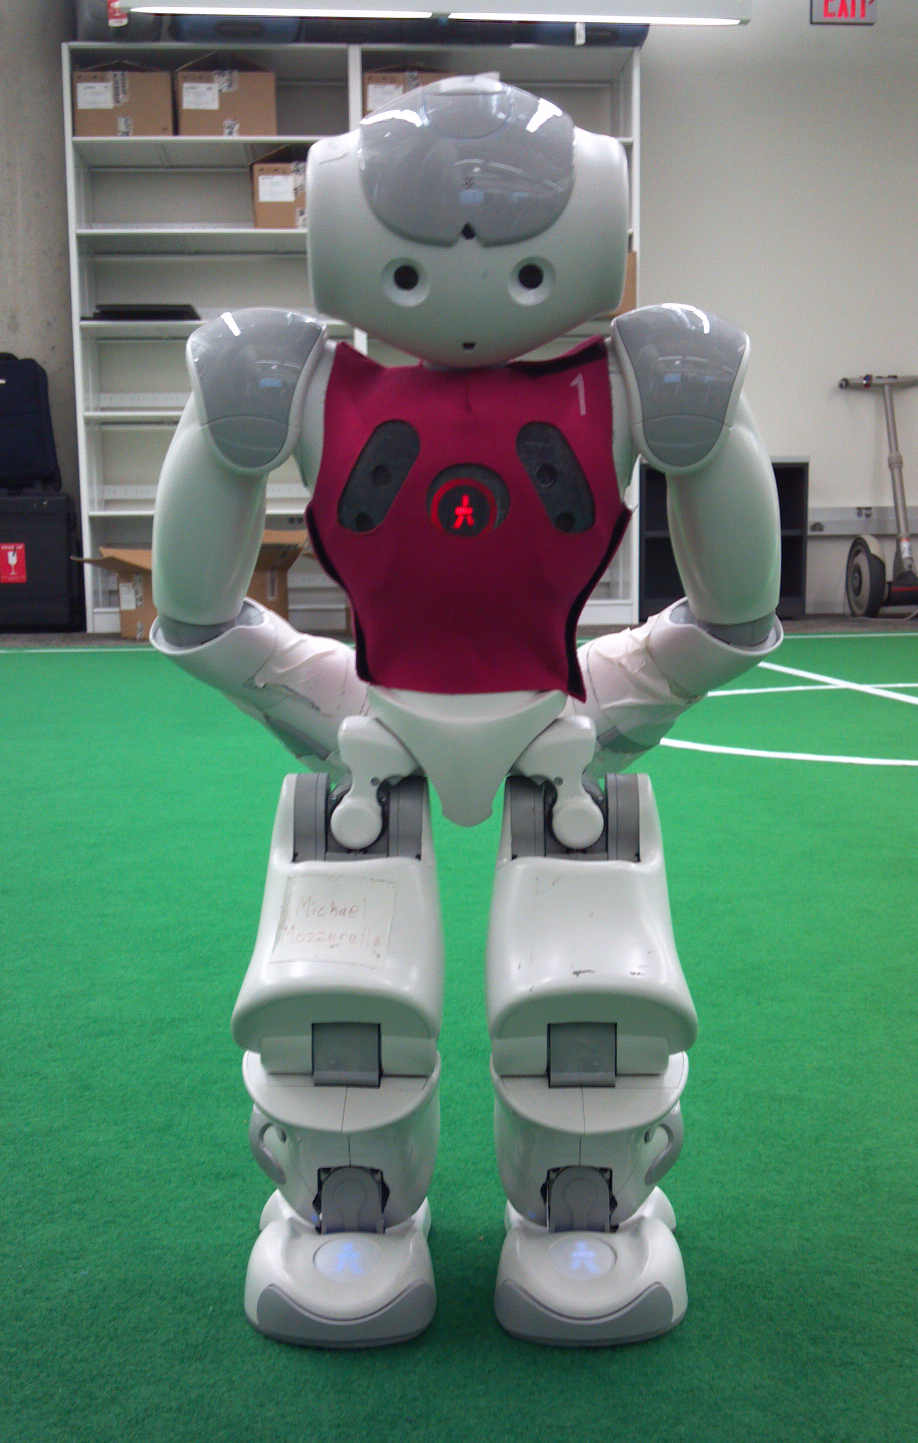
\includegraphics[height=0.28\columnwidth]{figs/front.jpg}&
      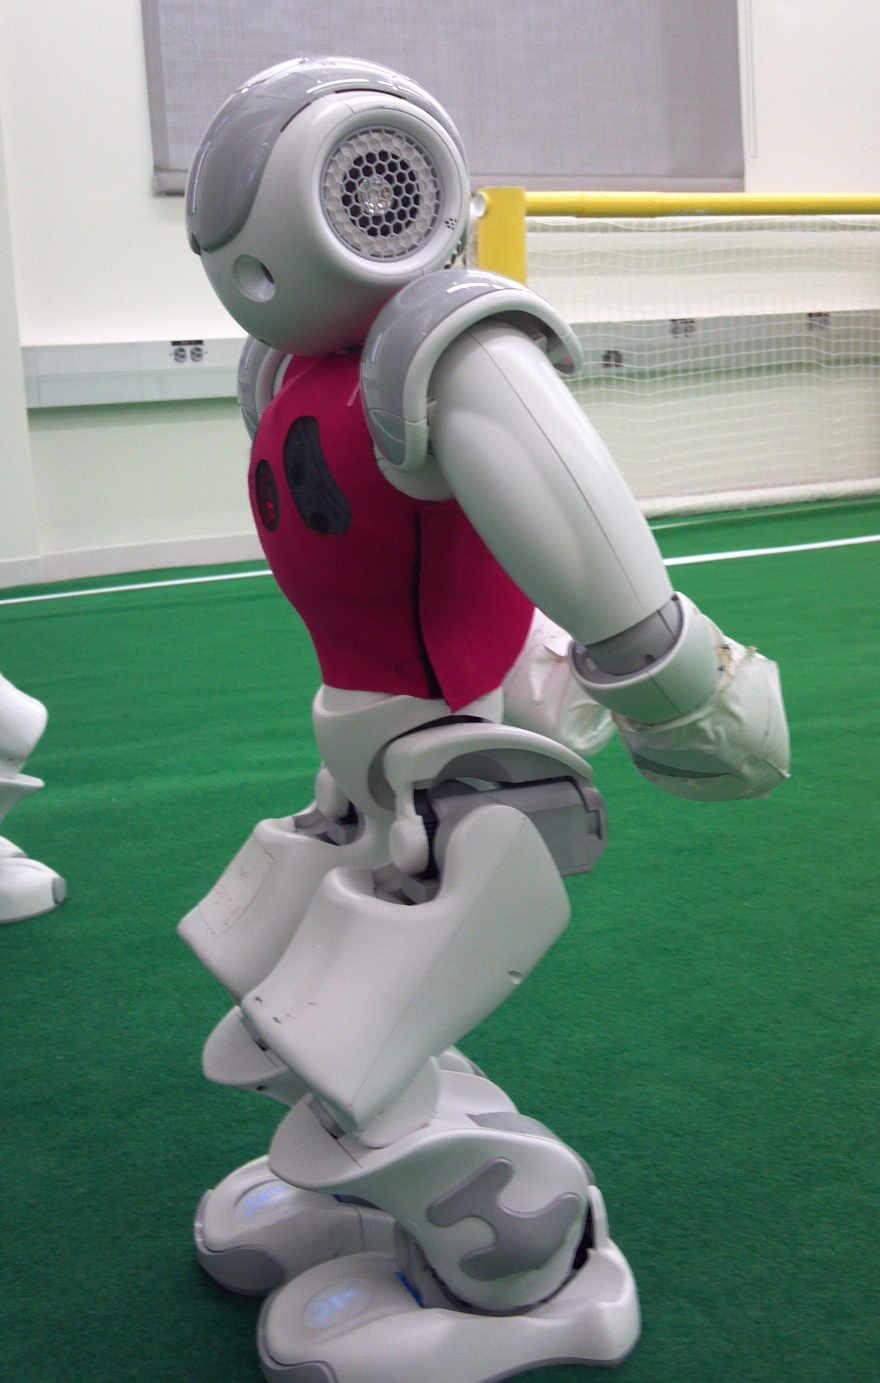
\includegraphics[height=0.28\columnwidth]{figs/side.jpg} &
      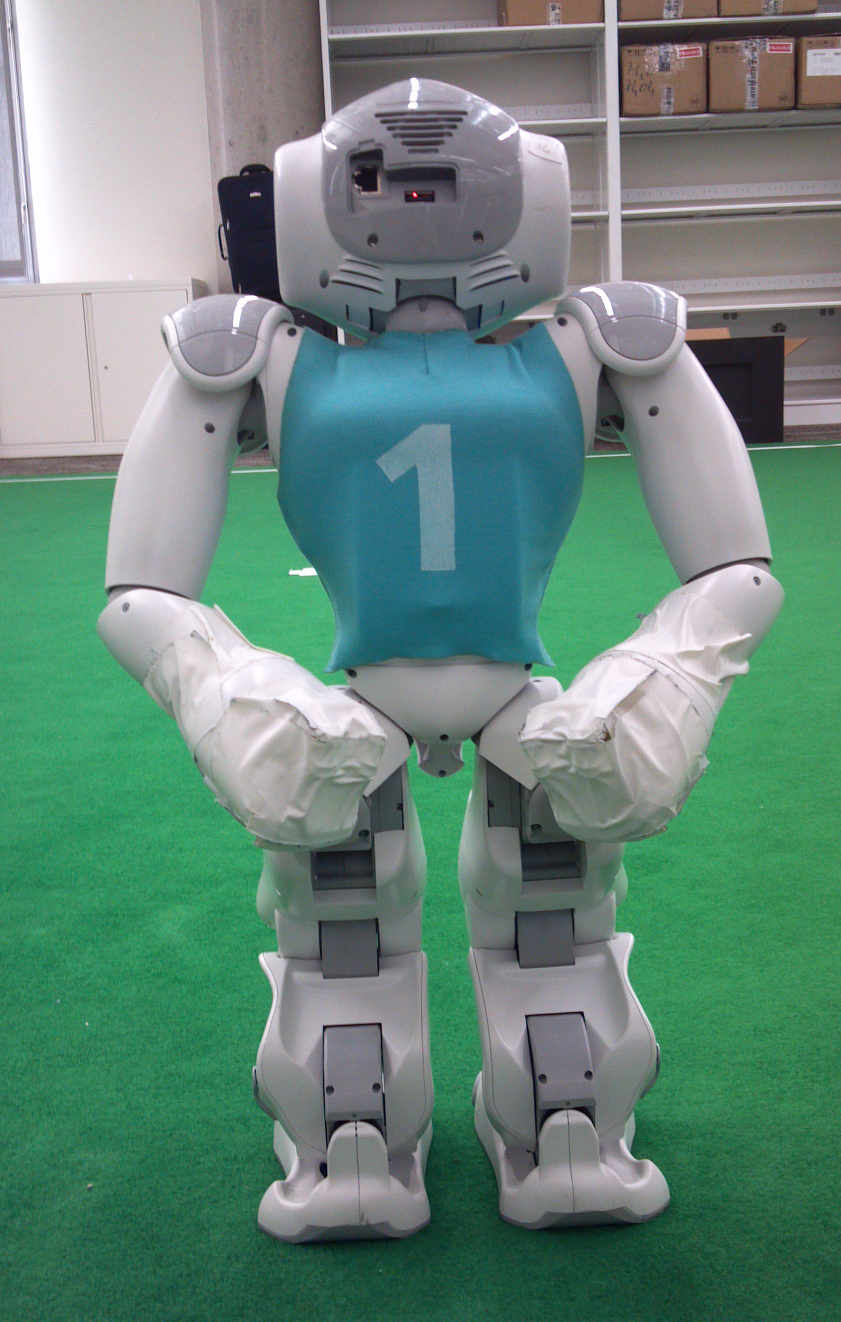
\includegraphics[height=0.28\columnwidth]{figs/back.jpg}
    \end{tabular}
  }
  \caption{Team markers. a) Front view. b) Side view. c) Back view.}
  \label{fig:nao_markers}
\end{figure}
Teams may use any jersey that was approved for a RoboCup SPL competition in the last 4 years without needing to approve it in \RCYear again.

Teams may design and manufacture their own jerseys in any color (multi and many color jerseys are acceptable), but must follow these guidelines:

\begin{itemize}
  \item Jerseys should be the \textbf{tank top} style used at RoboCup 2013/2014 and should cover approximately the same areas of the robot as shown in \cref{fig:nao_markers}.
    The torso LED must be clearly visible.
    Jerseys may include the sonar panel used in the 2013/2014 jerseys, although this is not required.
    Jerseys may not cover the shoulders of the robots.
  \item Jerseys must have a primary color that comprises more than half of the jersey.
    The primary color must be recognizable from the front and back.
  \item Jerseys should not contain distractors, such as large pictures of SPL balls or white stripes on green jerseys.
  \item A team must wear the jerseys that it starts a game in for the entire game.
  \item Jersey material must be non-reflecting and non-shiny.
    Material that is glittery is also not appropriate.
    Jerseys may be manufactured from fabric and fine mesh.
  \item Jerseys should be numbered 1--{\MaxJerseyNumber} on both sides.
    The numbers must be large and {\bf easily} recognized by humans.
  \item Teams must have two sets of jerseys for \emph{field players} that are significantly different in terms of their primary color.
  \item Teams must have two sets of jerseys for \emph{goalkeepers} that are significantly different in terms of their primary color.
    One of the \emph{goalkeeper} primary colors must be different from both primary colors used for \emph{field players}.
  \item Designs must be submitted to \url{rc-spl-tc@lists.robocup.org} for approval by \DTMdate{\JerseyApproveSubmissionDate}.
    If the team has jersey prototypes, they should submit close-up images of a robot wearing the jersey---these images should be taken from front, back, and side angles.
    If the team has no prototypes, then designs depicting the expected jersey should be submitted.
    If submissions show separated front and back halves of jerseys then the team must specify which halves are matched to form home and away jerseys.
    All images and designs should be submitted in pdf or jpg format.
\end{itemize}

The jersey sets that are used in a game are decided by the head referee in accordance with the teams during the pre-game meeting (\cf~\cref{sec:referee_team_communication}), subject to the following conditions:

\begin{itemize}
  \item Both teams' \emph{field player} colors must be easily distinguishable from each other.
  \item Both teams' \emph{goalkeeper} colors must be easily distinguishable from both teams' \emph{field player} colors.
  \item The two \emph{goalkeeper} colors may only be similar when this is the case for all choices among the available jersey sets.
\end{itemize}
The head referee should respect the teams' wishes unless they violate the above conditions, in which case the head referee must bring about a solution.

Some teams wish to include additional information or logos on their robots.
The following are allowable:

\begin{itemize}
  \item Adding sponsor or team logos to the upper legs of the robots (\cf \cref{fig:sponsor}).
    A box drawn around the non-white area of any logos must not cover more than a \qty{25}{\square\centi\metre} area.
  \item Adding small black and white stickers to the torso and/or head of the robots stating the name of the robot, the name of the team, or similar information.
    These stickers must be small and mostly white.
\end{itemize}

\begin{figure}
  \centerline{
    \begin{tabular}{ll}
      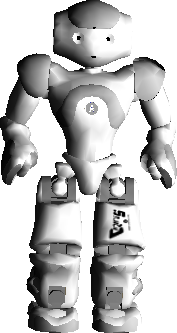
\includegraphics[height=0.35\columnwidth]{figs/naosim_with_logo.png}&
      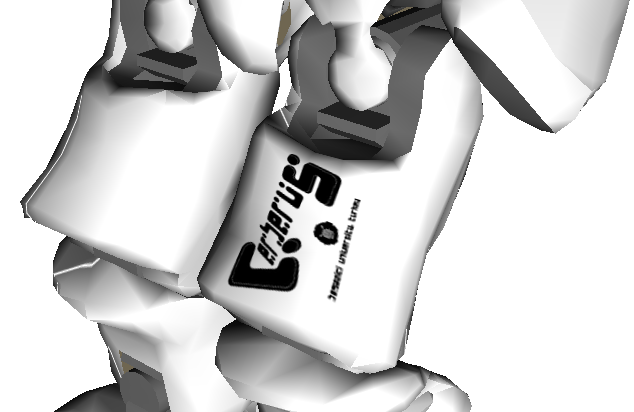
\includegraphics[height=0.35\columnwidth]{figs/naosim_legs_with_logo_closeup.png}
    \end{tabular}
  }
  \caption{Example Sponsor/Team Logo placement on legs.}
  \label{fig:sponsor}
\end{figure}

\subsection{Goalkeeper}
\label{sec:goalkeeper}

The \emph{goalkeeper} may use any of the allowed jersey numbers.
The \emph{goalkeeper} must wear a jersey with a primary color different from the primary colors used by the \emph{field players} of both teams.

\subsection{Communications}

The robots must play without human control.
Communication is only allowed among robots on the field and between the robots and the GameController.

\subsubsection{Non-wireless Communications}
\label{sec:acoustic}

In general there are no restrictions on communication between robots in play on the field using visual signalling (\eg gestures) or the robot's built-in microphones, speakers, and infrared transceivers.
However, communication that causes excessive discomfort to an audience, affects the safety of an audience, or violates normal playing rules is not permitted.

\subsubsection{Wireless Communications}
\label{sec:wireless}

The only wireless hardware allowed to be used by the teams are the wireless network cards built into the NAOs, and the access points provided by the event organizers.
All other wireless hardware must be deactivated.
A team may be disqualified if one of the team members violates this rule.

Each team will get a range of IP addresses that can be used both for their robots and their computers.
The network configuration (\eg IP addresses, channels, SSIDs, and required encryption) of the fields will be announced at the competition site.

Wireless robot-to-robot communication among the robot players is allowed, as long as it uses the access points provided by the event organizers (using the so-called ad-hoc mode is prohibited), messages are sent via UDP broadcast, and each message's payload size does not exceed \qty{\TeamMessageSize}{\byte}.
Each team will be allocated a single UDP port on which to send/receive their team messages.
Specifically, a team's port will be 10000 plus that team's GameController number.
Unicast communication between robots is prohibited.

The amount of data transmitted by a team in a single game is limited.
The limit is measured as the total number of UDP packets sent by any robots of a team.
A team may not exceed \qty{\TeamMessageLimit}{packets} per game.
For each minute of irregular extra time (\cf~\cref{sec:extra_time}), the limit is increased by \qty{\TeamMessageLimitMinute}{packets}.
However, this does not apply to a team that has already exceeded its limit before.
The GameController tracks the number of messages that have already been sent and includes counters for packets remaining per team in \texttt{RoboCupGameControlData}.

If a team exceeds their limit the game is scored with 0 goals for the offending team.
Robot-to-robot communication that violates the SPL rules result in a game scored with 0 goals for the offending team (even when discovered after the game was finished).
Messages are counted towards the limit during the \texttt{standby}, \texttt{ready}, \texttt{set} and \texttt{playing} states.
Limits do not apply during penalty kick shoot-out.
If a knock-out game results in a draw and both teams exceeded their message limit, the team last exceeding their limit wins the game.

The limit of allowed packets will be lowered in future competitions to encourage smart event-based communication.

In addition to robot-to-robot communication, robots may send:
\begin{itemize}
 \item Additional status update packets that are sent to the GameController.
 \item Team specific debug information may be sent to an external computer owned by the team.
   A robot may send debug information at most once every \qty{2}{\second} in a single UDP packet.
\end{itemize}
These additional packets do not count towards the team's data limit and may not be used for robot-to-robot communication.
They must be sent as unicast and may not be sent as broadcast.

Teams and their robots must not listen into another team's communication.

Robots are not allowed to be connected to access points of fields that are currently running official games of other teams.
Robots may only communicate on fields that are not running an official game or fields which they are playing on.

The GameController will use UDP to connect to the robots.
The source distribution of the GameController provides the header file \emph{RoboCupGameControlData.h} that defines all messages sent by the GameController to the robots.
They correspond to the \emph{robot states} described in \cref{sec:robot_states}.

Robots send status updates (defined in \emph{RoboCupGameControlData.h}) to the GameController.
These return packets must be addressed directly to the GameController PC (\ie not broadcast) and sent on the GameController return UDP port specified by the symbol \verb!GAMECONTROLLER_RETURN_PORT! in \emph{RoboCupGameControlData.h}.
The rate at which return packets may be sent is limited to \qty{2}{\per\second}.

The use of remote processing/sensing is prohibited.
